\section{Methodology}

For the realization of our concept, we aimed for the accomplishment of the following three objectives:

\begin{enumerate}
    \item Obtaining a sufficiently large dataset with different expressions about the topic of AI.
    \item Raw data transformation into a dataset that matches the target schema illustrated in \autoref{fig:overview}.
    \item Creation of a visualization from which society's perceptions on different topics of AI can be extracted.
\end{enumerate}%
%
%
\begin{figure}[t]
    \centering
    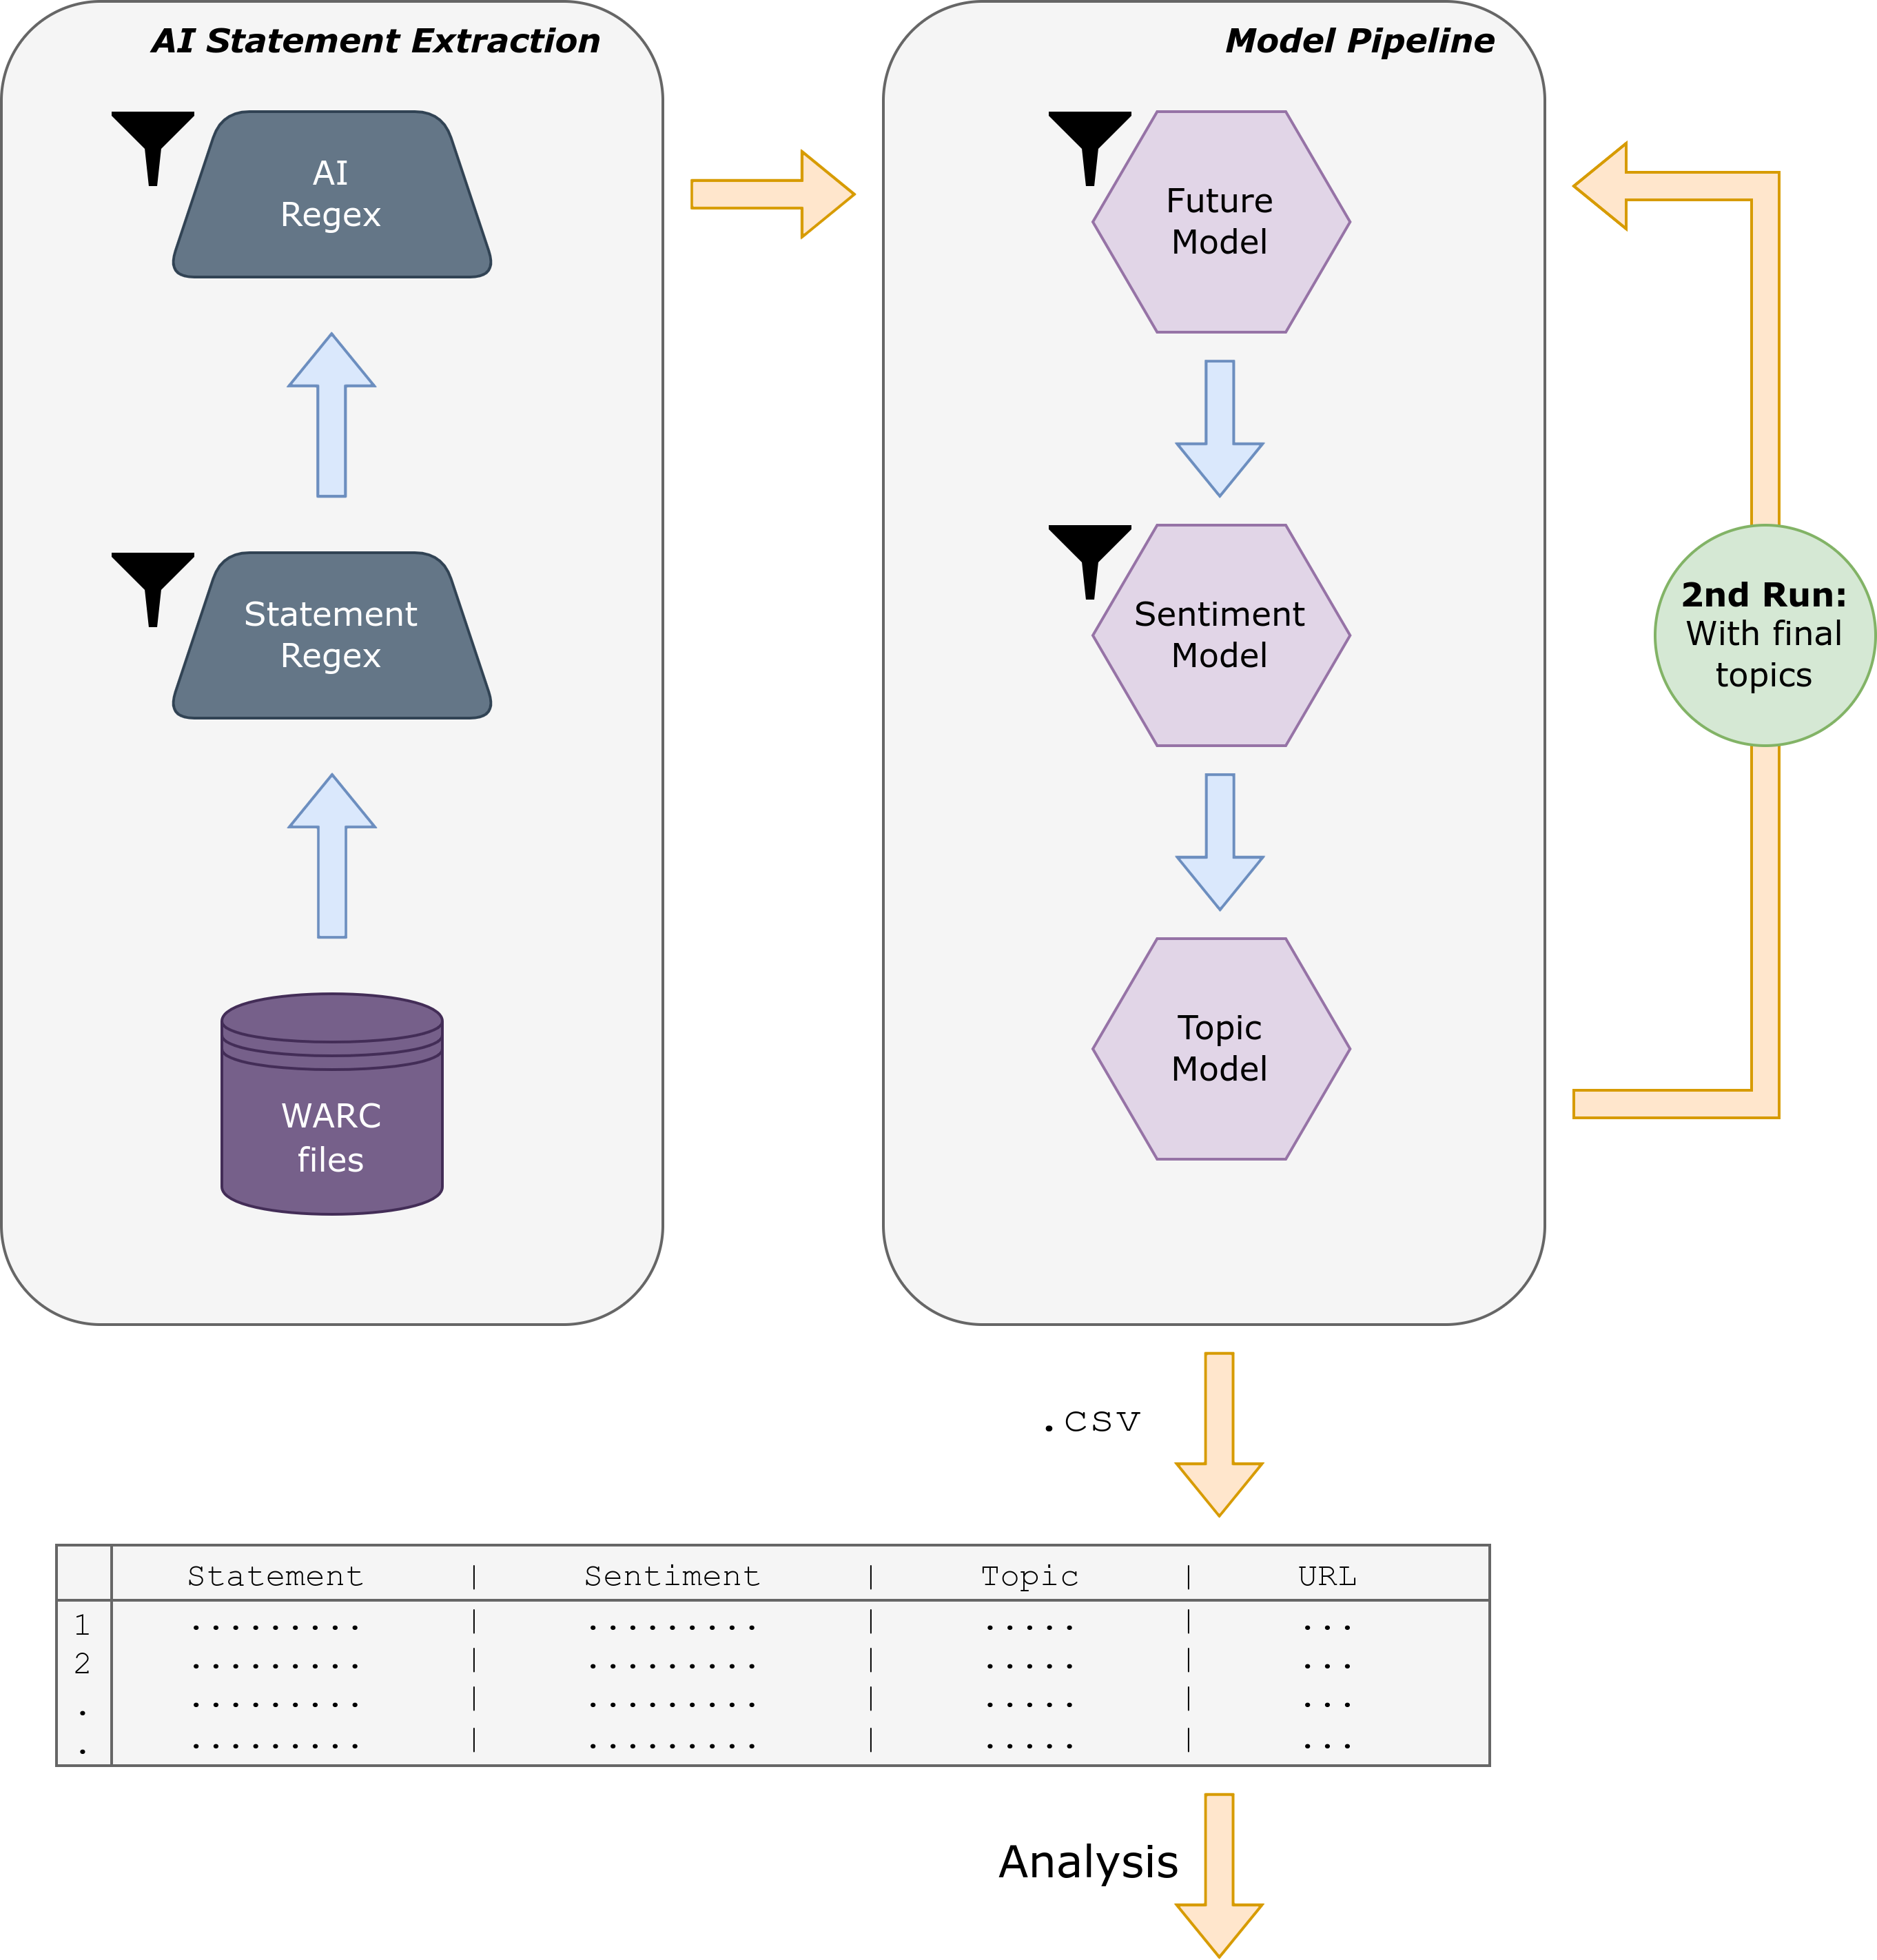
\includegraphics[width=\linewidth]{overview}
    \caption{
        The statement extraction, filter and final topic assignment process.
        AI statements are extracted from website HTMLs located inside WARC files (left part).
        The extraction process involves the application of two regexes (statement regex and AI regex).
        Statements then enter the model pipeline (left side), where they are further filtered through the future model and the sentiment model.
        The model pipeline runs two times in total. The first time the topic model assigns dummy topics.
        After the topic selection process (green circle), where we fine-tune the topic model, the model pipeline runs a second time.
        Now the topic model assigns the final topics to the statements.
        The output is a CSV file with the schema \texttt{statement|sentiment|topic|url}.
    }
    \label{fig:overview}
\end{figure}
\underline{1. WARC Data Extraction:}
\\
Initially, we outline the raw data acquisition containing AI expressions.
Since a web archive with the corresponding WARC-DL data extraction pipeline \citep{Deckers2022} was at our disposal, we utilized both.
Sentences about AI can be extracted for later processing by applying Regular Expressions (Regex) on every sentence of the data.
\\
\\
%
\underline{2. Data Transformation:}
\\
For later analysis, the data had to be converted into the required target schema, illustrated in \autoref{fig:overview}.
Therefore, we created a model pipeline which generates the final dataset with the attributes future statement, sentiment, topic, and URL.
Three sequential models are applied within this model pipeline:
\begin{itemize}
    \item Future Statements Model:\\
    This model is able to distinguish between statements about the future and all other types of statements.
On the basis of its classifications, we only extracted statements about the future.
    \item Sentiment Model:\\
A sentiment is assigned to every future statement by this model.
    \item Topic Model: \\
    Before our topic model of choice is able to assign  reasonable topics to our statements, those had to be provided to it as label candidates.
Accordingly, the Model Pipeline runs twice. In the first execution the chosen model runs with dummy topics. Based on the output, the topic selection is conducted.
For each subsequent run, the model pipeline is considered complete.
\end{itemize}%
%
The resulting dataset can then be used for analysis and interpretation.
\\
\\
\underline{3. Analysis:}
\\
For our analysis, we start with a graphical visualization.
Therefore, we decided to group all statements according to their topics so that a sentiment analysis could be conducted for each topic separately.
\\
\\
In the following sections, each step of the implementation is discussed in detail.


\subsection{WARC Data Extraction}
The Webis Group\footnote{\url{https://webis.de}} had granted us  access to 37,908 Web ARChive (WARC) files and a high-performance computer cluster on which we were able to schedule jobs.
Additionally, we decided to utilize the WARC-DL pipeline \citep{Deckers2022}, a Python software pipeline tightly coupled with the WARC endpoint, and to use the FastWARC\footnote{\url{https://resiliparse.chatnoir.eu/en/stable/man/fastwarc.html}} library for iterating over WARC records under the hood.
It enabled us to automatically extract text  from the WARC records using several customizable filters.
We made some slight modifications to the source code to make it fit our needs better.
\\
To find all statements on a website related to AI, we first built a Regex pattern to cut text from an HTML source. A second Regex pattern then extracted statements containing one or more AI keywords from this text. Since we wanted to analyze AI statements, we did not need all the text provided by a website HTML, but only full sentences of the English language. 
As it proved impossible to extract all statements with a 100\% accuracy using Regex only, we narrowed our filter down to passages which started with a capital letter and ended with a period or exclamation mark.
\\
\\
Additionally, since initial runs of the WARC-DL pipeline included large amounts of inappropriate content (including content in languages other than English), we created a whitelist to only accept the most common English language top level domains and a blacklist for filtering out domain names related to adult-content websites. 
\\
Due to problems with the cluster and WARC-DL pipeline, we could not extract all statements in one job run; jobs would suddenly stop because of connection errors or out-of-memory errors, and halt with exceptions. To overcome this issue, we separated hostnames in four groups depending on the initial hostname character: \texttt{a-h}, \texttt{i-p}, \texttt{q-x} and \texttt{yz0-9}.
This allowed us to pinpoint the problematic websites more precisely. In the end, we managed to extract data from all WARC files in group \texttt{i-p} and \texttt{yz0-9}, and most of the WARC files in groups \texttt{a-h} and \texttt{q-x}.
The final yield of the WARC data extraction stage was a total amount of 222,246 AI statements.
In the next steps, starting with the model pipeline, our objective was to further refine this initial data set.

\subsection{Model Pipeline}
\label{model-pipeline}
The model pipeline followed the WARC data extraction step and was designed to prepare our final dataset of future statements and their associated sentiment and topic labels. We performed the processing within the model pipeline on batches of 30 records each from the WARC-DL output. 
\\
First, the future model filtered out future statements from the corresponding batch. Subsequently, the chosen sentiment model assigned a sentiment to each future statement. In this step some future terms could be sorted out. This concerns the statements to which a sentiment was classified with a probability of less than 70\%. The remaining future statements received a topic. Finally, those were persisted in a CSV file.
\\
The following sections \ref{future-model} - \ref{topic-model} will go into detail about each individual model.
In this context, we describe how the future model was trained and justify our decision for the sentiment and the topic model selection.
Furthermore, we outline the choice of our topics and explain, why only those statements are kept which a sentiment with a probability above 70\% can be attributed.

\subsection{Future Model}
\label{future-model}
Since this paper focuses on analyzing statements about the future, a system for distinguishing between future statements and other expressions is required.
In this context, we decided to finetune the DistilBERT \citep{Sanh2019DistilBERTAD} base model that accomplishes this task.
Therefore, in this subsection, we thematize the collection of appropriate training data and the subsequent finetuning of the corresponding model.

\subsubsection{Training Data Set}
\label{training}
To collect suitable data for training the Future Model, we needed a balanced dataset containing statements classified as addressing the future and all other, non-future statements. We therefore adopted multiple approaches.
In order to increase diversity and reduce bias, two of our group members manually annotated 500 observations each, while the other two built an automated mechanism with subsequent verification.
\\
One of the automatized approaches involves a web crawler developed on the basis of the python library Beautiful Soup \citep{Richardson2022}.
It works by dividing the text on a page into sentences.
Subsequently, every sentence is examined for occurrence of certain terms, such as \emph{going to}, \emph{will}, \emph{won't} or \emph{'ll}.
\\
The second automated approach is a sentence extraction tool, which works similar to the web crawler in several aspects.
At the beginning, it searches the given directory for text files.
If those exist, the text is split into sentences and observed for specific expressions, as described above.
\\
To find the phrases that are not future statements, both the web crawler and the sentence extraction tool look only at the corresponding records that do not contain the previously considered expressions.
A careful manual review of all terms gathered by the automated systems was subsequently performed to remove the incorrect records.
\\
Finally, we constructed a dataset with 1,250 future statements and 1,250 other phrases that did not contain future statements.

\subsubsection{Training}
As previously described, we used the DistilBERT base model and finetuned it with the data set specified in \ref{training}.
We split the dataset of 2,500 records into a training and a test set, where the test set contained 20\% of the records.
From the training set we further split 20\% for validation data.
\\
After only two epochs the training ended with an accuracy over 96\% as displayed in \autoref{future-model-train}.
\\
Following, we tested the model on our test set containing 500 records never seen by the model and achieved an accuracy of 93.8\%, as seen in the confusion matrix in \autoref{fig:cm}.


\subsection{Sentiment Model}
In order to assign sentiments to future statements for later analysis, we decided to select a pre-trained model.
The chosen sentiment model is the SentimentAnalyzer of the open-source library pysentimiento \citep{perez2021pysentimiento}, which was further trained on about 40,000 tweets.
It uses the BERTweet \citep{bertweet} model as a base model, pre-trained on English language tweets.

\subsubsection{Evaluation}
To evaluate the SentimentAnalyzer, we annotated 604 future statements, previously used for training the future model, as negative, positive or neutral and received an accuracy of about 65\%.
\\
We then analyzed all misclassified statements and noticed that some of them could not be assigned impartially to one of the three categories.
An example is \emph{``AI will reinvent how we think about education''}.
In the case of this sentence, we disagreed on whether we should value the sentence as neutral or positive and decided to use the neutral label.
However, this statement was given a positive rating by the model.
On closer examination of the statements that were labeled differently by us and by the model, we found over 90\% of the labels given by the model to be valid, if these annotations had a probability of correctness over 70\%.
For this reason we decided to only keep statements about the future which the sentiment model had annotated with a confidence above 70\%.

\subsection{Topic Model}
\label{topic-model}
\begin{figure}[t]
    \centering
    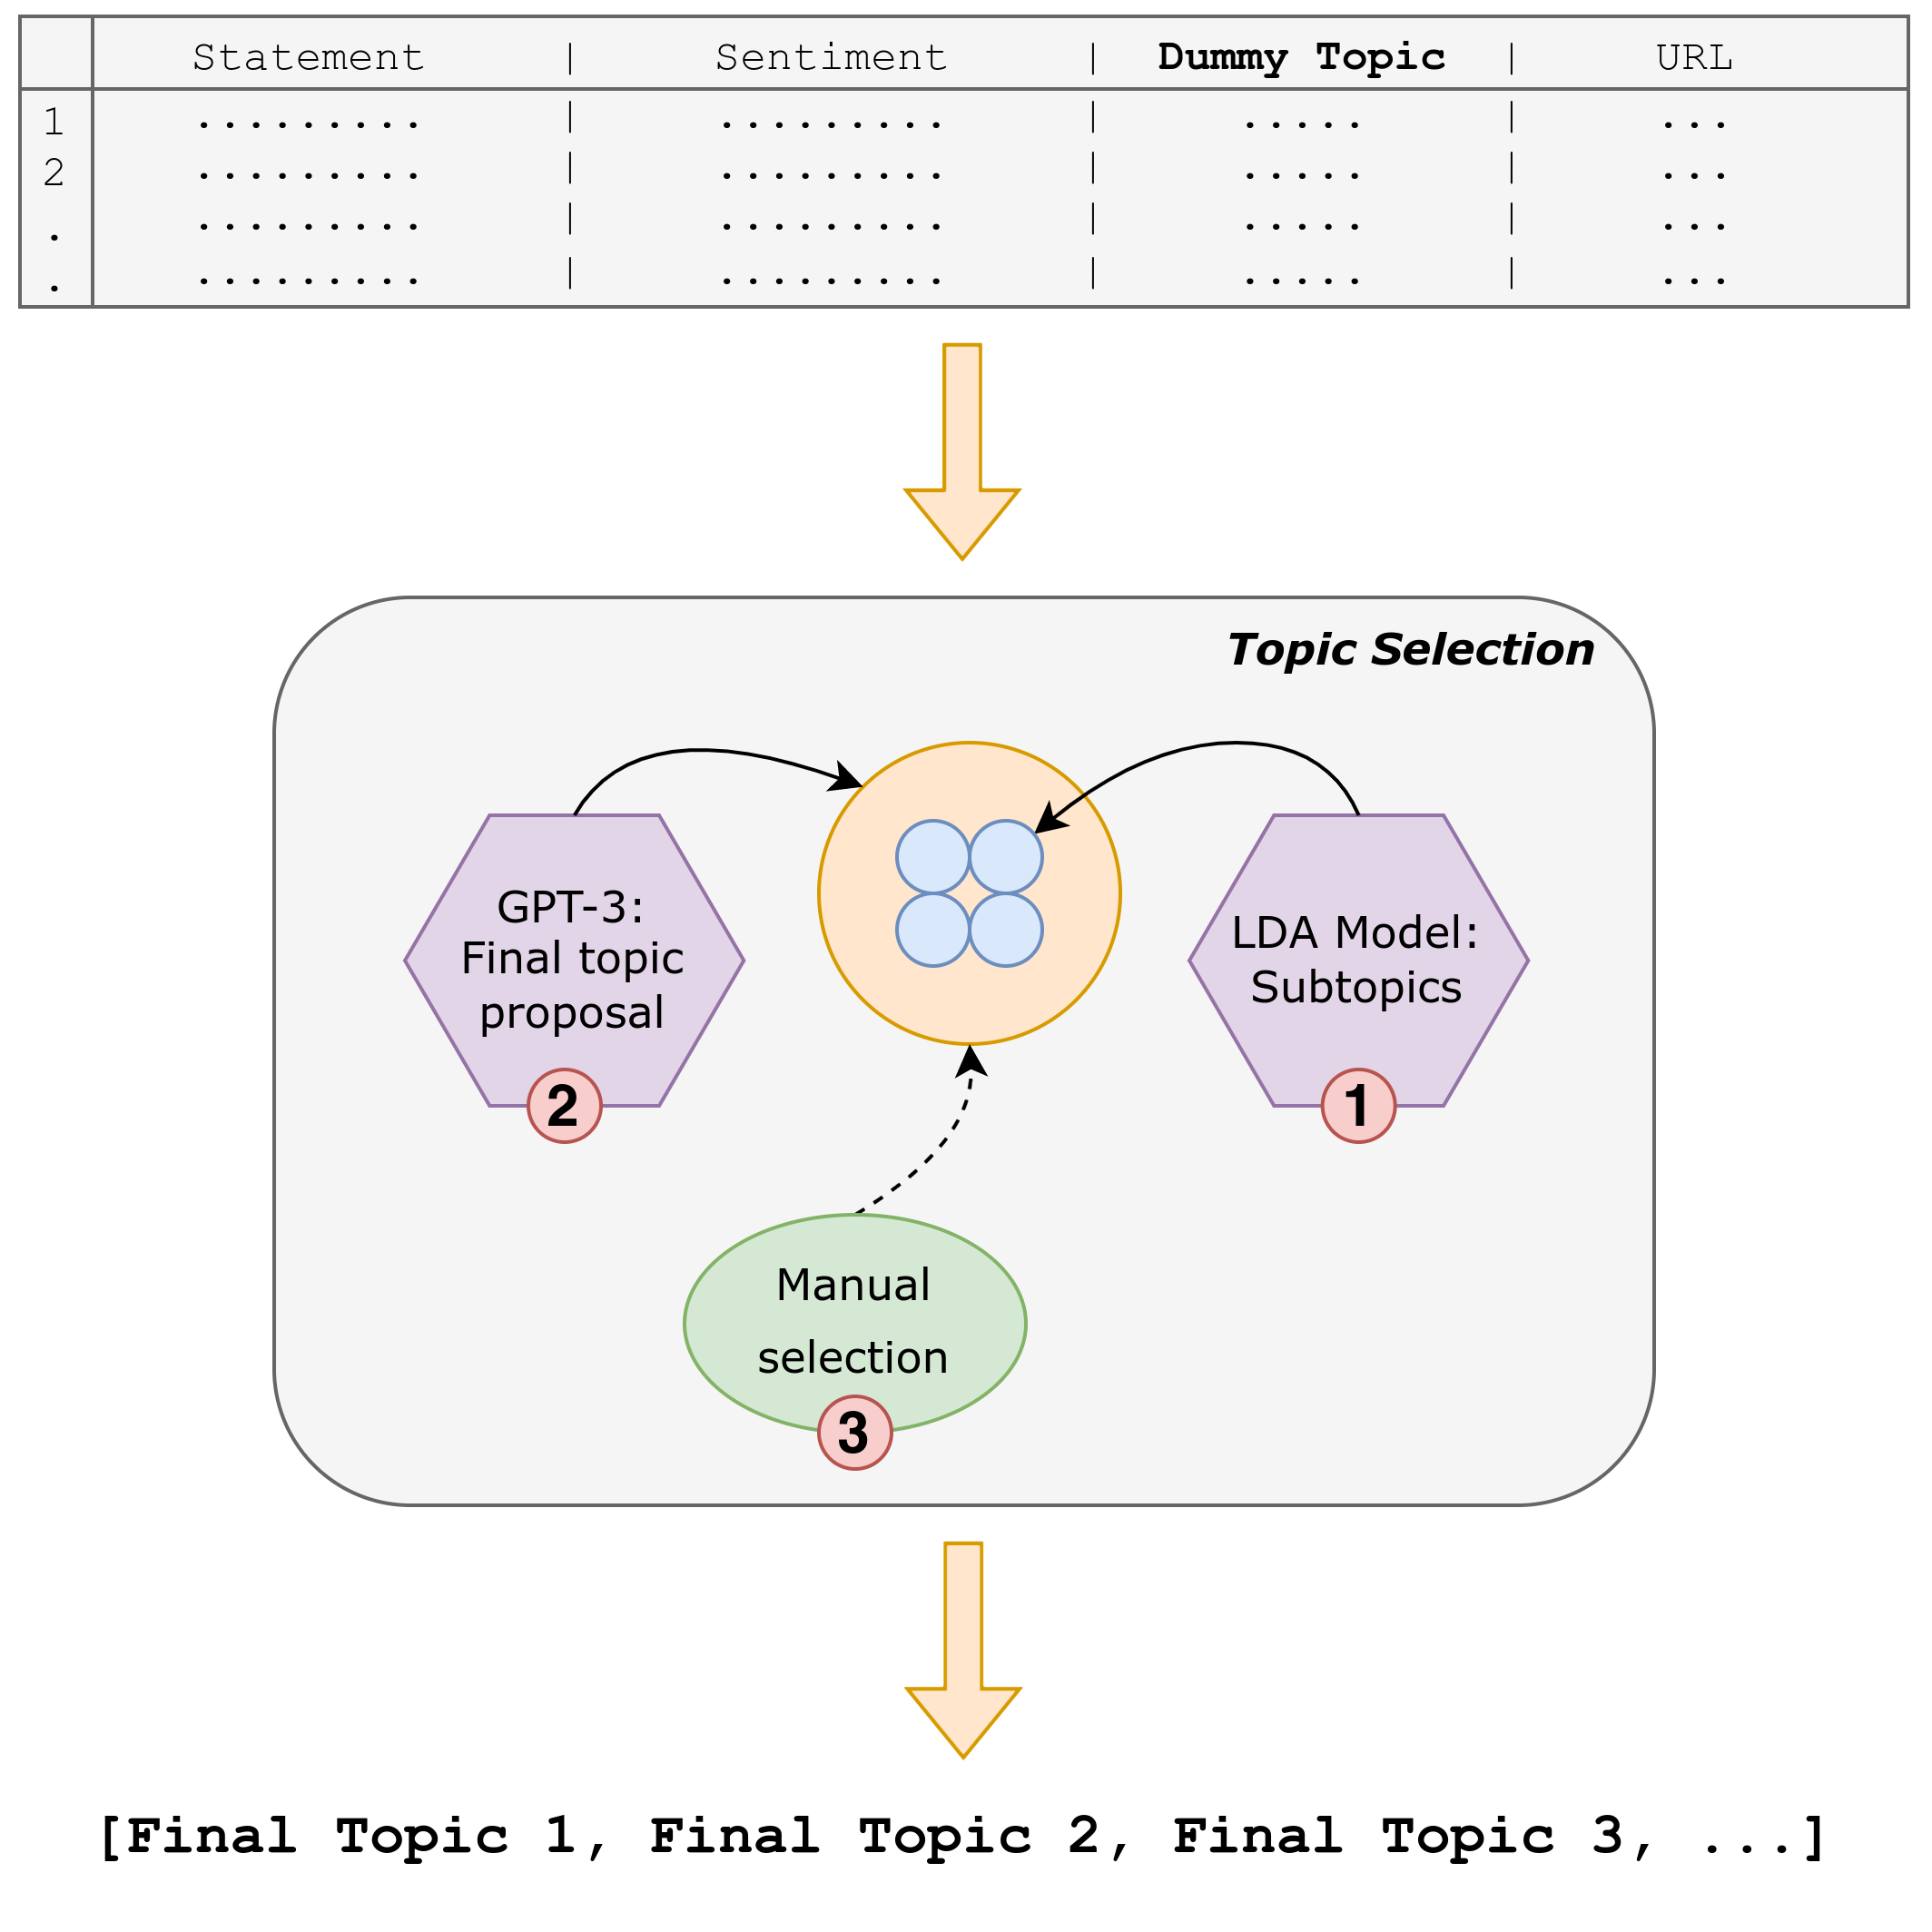
\includegraphics[width=\linewidth]{topic_selection}
    \caption{
        The three steps of topic selection.
        First, the LDA Model generates a set of subtopics for a topic cluster.
        In this example, there are four subtopics (small blue circles).
        Then, GPT-3 proposes a possible general topic for the subtopic set (large yellow circle).
        Lastly, we either pick this final topic as proposed, or replace it with a more suitable one from the same category, e.g. \texttt{level} would become \texttt{gaming}.
    }
    \label{fig:topic_selection}
\end{figure}
For assigning topics to the future statements we employed the bart-large-mnli model from Facebook, which was pre-trained on the MultiNLI \citep{N18-1101} dataset, which consists of 433,000 pairs of sentences annotated with textual supplementary information. The bart-large-mnli is a natural language processing model based on the technique of \citet{yin2019benchmarking} utilizing pre-trained NLI models as ready-to-use zero-shot sequence classifiers.
The approach involves specifying the sequence for classification as an NLI prerequisite and then constructing a hypothesis of every possible label candidate.
Afterwards probabilities of agreement and contradictions are transformed into annotation probabilities.
Before we were able to use the bart-large-mnli, however, it was necessary to define the topics, which could be assigned to every statement by this model.
For instance, to verify whether a sentence was a political or a technological statement, we could provide the model with the label candidates: \emph{politics} and \emph{technology}. Then the model would apply one of the labels to the sentence.
The following section describes our topic selection approach in detail.

\subsubsection{Topic Discovery with LDA}
\label{lda}
For analyzing the overarching topics within our future statements, we used Latent Dirichlet Allocation (LDA). LDA is a subtype of the Dirichlet Process Mixture Models (DPMMs), a set of non-parametric, “fully-Bayesian” unsupervised clustering models which are commonly used for topic cluster analysis. DPMMs use a stochastic process to generalize the Dirichlet distribution (the conjugate prior for a categorical or multinomial distribution) for infinitely many categories \citep{li2019tutorial}.
Applied to NLP, a Latent Dirichlet Allocation model clusters observations into unobserved groups of related data. It has the advantage of following a generative process that is immune to overfitting with increasing size of the data corpus and can be scaled to a data cluster in machine learning \citep{pritchard2000inference}.
\\
\\
We preprocessed our dataset for LDA.
From there on, we created bigrams (sets of two words) from the tokens and employed a Word2Vec model to select only the most frequently occurring ones.
Afterwards, bigrams that occurred in more than 60\% statements and less than 20 of the documents were filtered out. The remaining bigram candidates were fed into an LDA model, returning clusters of related topics. To label each cluster with a matching headline or cluster name, we used OpenAI’s GPT-3 (text-davinci-002) to turn suggestions of cluster names.
\\
Inspired by these suggestions, we chose topic names that we considered the best fit for for every cluster of topics.
Eventually, with this approach we received the following headings for our Topic Model: search engine, finance, transhumanism, machine human interface, social media, search engine, and natural language technologies.


\subsection{Analysis}
For the analysis of the previously created dataset in \ref{model-pipeline}, we focused on the attributes topic, subtopic, network, and sentiment of each tuple.
Since the future dataset generated by the Model Pipeline only captured the topic or category of a future statement and the sentiment attribute, we included further subtopics.
To accomplish this, we proceeded as described in section \ref{lda}.
Consequently, the resulting data for every statement contained not only a topic but also a subtopic.
This way we intended to analyze each future statement category in more detail.
To accomplish this we extracted the original subcategory list of each topic utilizing the LDA model and combined these lists to a single one. We aimed to find a subtopic for almost every statement.
Therefore, we checked whether a statement contained a subtopic from the list and selected the first one.
To obtain the most suitable assignment of subtopics to statements, we maintained the order of these subcategories within each original list.
In conclusion, the more meaningful statement subtopics found by the LDA model were prioritized. Sentences that did not contain any of this subtopics were marked as 'undefined'.
This way, we were able to obtain the average sentiment scores for each theme and subcategory.
\\
\\
Furthermore, we added a number to every statement, mapped to every statement for a later sentiment score calculation. To negatively perceived sentences we assigned a \texttt{–1}, while positively labeled terms receive a \texttt{1}. Finally, every statement containing a neutral sentiment obtains a \texttt{0}.
